\section{Introduction to Neural Networks}

Neural Networks are a type of a machine learning model inspired by activities in human brain.
A neural network comprises of `neurons`, which are considered as the building blocks.
A neuron in a neural network is implemented as weighted sum of its input, which is then passed through a non-linear function. This non-linear function is often denoted as an activation function and most commonly is a sigmoid or a rectified linear function.

Let $W$ be weights and $x$ denote the inputs. Let $g$ be the activation function, then a single neuron is represented as - 


\begin{figure}[H]
   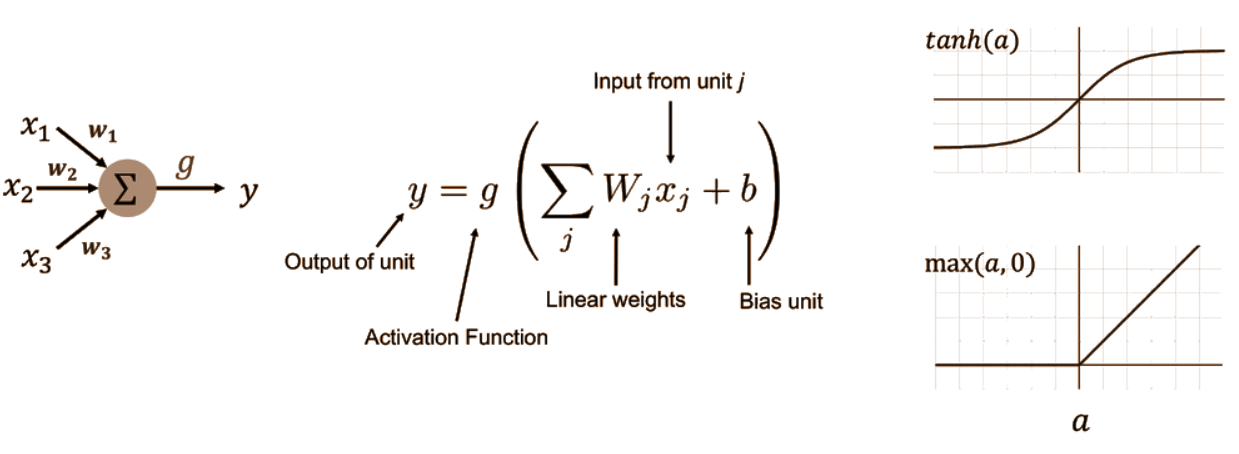
\includegraphics[width=1\linewidth, scale=0.9]{figures/intro/neuron.png}
   \caption[Artificial Neuron]{Artificial Neuron and common activation functions}
    \label{fig:neuron}
\end{figure}


When multiple of neurons are connected in a layer to all the inputs and the output of these neurons are used as input to another set of neurons, then the structure is called as Neural Network. This is shown in the figure ~\ref{fig:ann}. In this network $x_1$ and $x_2$ are the inputs to the network. $f_1(e)$, $f_2(e)$ and $f_3(e)$ are the outputs of three neurons in the first layer. They form as the inputs to the second layer. Simillarly $f_4(e)$ and $f_5(e)$ are the outputs of second layer and $f_6(e)$ is the final output which is used to predict the final value - $y$.


\begin{figure}[H]
	\centering
   \includegraphics[scale=0.66]{figures/intro/neural_network_start.bmp}
   \caption[Artificial Neuron]{Artificial Neuron and common activation functions}
   \label{fig:ann}
\end{figure}

\subsection{Learning}

Learning of Neural Networks is done in four steps --

\begin{enumerate}
	\item Forward pass

During the forward pass the outputs are computed by multiplying the weights $w$ with the inputs (x). Let $w \times x$ be denoted as $e$ and the activation function be denoted as $f$, then output of a layer $f(e)$ would be $f_1(w_1 \times x_1 + w_2 \times x_2)$. 
If we consider the network shown in figure ~\ref{fig:ann}, then a single forward pass would be as depicted in the figure ~\ref{fig:forward}.

\begin{figure}[H]
	\centering
   \includegraphics[scale=0.66]{figures/intro/forward.bmp}
   \caption[Forward pass]{Computation of a forward pass in a neural network}
   \label{fig:forward}
\end{figure}

	\item Compute error

Error is computed once the model has predicted its output ($y$). Let $z$ be the true output for the given data points. 
Error function or the loss function takes in the predicted value ($y$) and the true value ($z$) and returns some numeric value.
This function is task specific and is different for different tasks. For simplicity let's assume a simple difference, then the error $\delta$ is $z-y$, as shown in the figure ~\ref{fig:error}.

\begin{figure}[H]
	\centering
   \includegraphics[scale=0.66]{figures/intro/error.bmp}
   \caption[Compute error]{Computation of error in a neural network}
   \label{fig:error}
\end{figure}


	\item Backward pass

Backward pass is a phase where error with respect to every neuron is computed. Error at a given layer is the proportion of the error contributed by that layer wrt to the total error. In order to compute error for layer $l$ we need to know error at layer $l+1$. 
Thus, it is computed from layer layer to the first layer and hence called Backward pass. For the networks shown above, error at neuron $2$ is weighted sum of errors at neuron $4$ and $5$. This is shown in the figure ~\ref{fig:error2}.

\begin{figure}[H]
	\centering
   \includegraphics[scale=0.66]{figures/intro/error2.bmp}
   \caption[Backward pass]{Backward pass of the error in a neural network}
   \label{fig:error2}
\end{figure}


	\item Weight update

Final step is to use the error at each neuron to change the weights. Current weight is changed by product of three values - error at the current neuron ($\delta$), gradient of the output wrt to the input at that node ($\frac{df(e)}{de}$)and the output $y$. Generally, this update value is too large and needs to be scaled. This scaling parameter ($\eta$) is called as the \textbf{learning rate} and is generally a hyper-parameter of the network. This step is shown in the figure ~\ref{fig:weight_update}.

\begin{figure}[H]
	\centering
   \includegraphics[scale=0.66]{figures/intro/weight_update.bmp}
   \caption[Weight Update]{Update of weights in a neural network}
   \label{fig:weight_update}
\end{figure}


\end{enumerate}

\section{Introduction to Convolutional Neural Networks}

Convolutional Neural Network are like standard neural networks except that not all neurons are connected to every input. 
Only local neighbourhood of inputs are shared for some set of neurons as depicted. Figure ~\ref{fig:cnn} shows the difference between standard Neural Networks (left) and Convolutional Neural Neworks (right).

\begin{figure}[H]
	\centering
   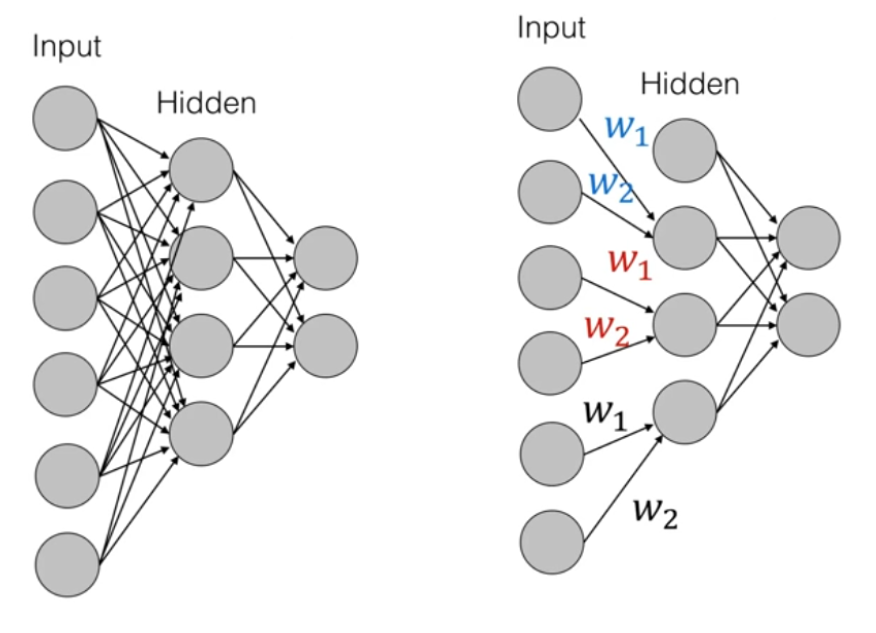
\includegraphics[scale=0.66]{figures/intro/cnn.png}
   \caption[Convolutional Neural Network]{Difference between Standard NN and Convolutional NN}
   \label{fig:cnn}
\end{figure}
